\section{Punto de Vista Físico}
\subsection{Modelo Físico}
\begin{figure}[h!]
	\centering
	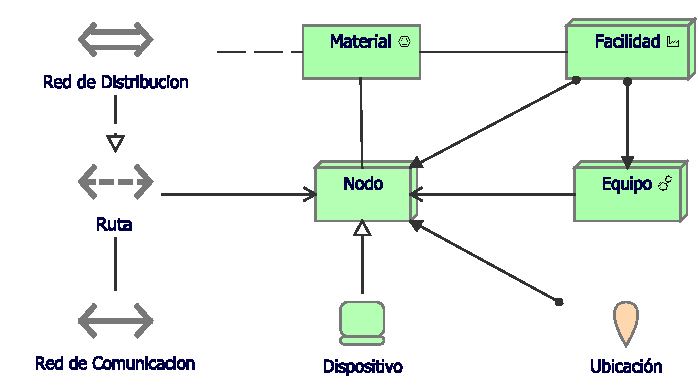
\includegraphics[width=.9\linewidth]{imgs/modelo/Fisico}
	\caption{Modelo Físico}
\end{figure}

El punto de vista físico es importante para los proyectos a realizar a escala industrial, no por el hecho de que sea fundamental para la construcción del proyecto sino más que todo es para su puesta en marcha. Como es bien sabido, todos los proyectos se realizan con alguna razón de ser, generalmente para cumplir una necesidad y/o ayudar a la comunidad con una función en específico, teniendo en cuenta esto, para la implementación y puesta en marcha del proyecto, es necesario tener en cuenta el punto de vista físico si el proyecto  así lo requiere.

Para el caso del proyecto Tu-Perfil, este no requiere un punto de vista físico como tal, puesto que no cuenta con los requisitos para que este exista, no se va a construir a gran escala o a escala industrial y todos los servicios que brinda este proyecto son digitales, por lo tanto aparte de las herramientas de computación y servidores no se requiere más indumentaria física.

\clearpage
